\documentclass[a4paper]{jpconf}

\usepackage{graphicx}

\usepackage{lineno}
\linenumbers

\begin{document}

\title{DAQExpert - An expert system to increase CMS data-taking efficiency}

\author{J-M Andre\textsuperscript{5}, U Behrens\textsuperscript{1}, J Branson\textsuperscript{4}, O Chaze\textsuperscript{2}, S Cittolin\textsuperscript{4}, C~Contescu\textsuperscript{5}, G-L Darlea\textsuperscript{6}, C Deldicque\textsuperscript{2}, Z Demiragli\textsuperscript{6}, M Dobson\textsuperscript{2}, N~Doualot\textsuperscript{5}, S Erhan\textsuperscript{3}, J R Fulcher\textsuperscript{2}, D~Gigi\textsuperscript{2}, M Gladki\textsuperscript{2}, F Glege\textsuperscript{2}, G~Gomez-Ceballos\textsuperscript{6}, J~Hegeman\textsuperscript{2}, A Holzner\textsuperscript{4}, M Janulis\textsuperscript{2,a}, M~Lettrich\textsuperscript{2}, F~Meijers\textsuperscript{2}, E Meschi\textsuperscript{2}, R K Mommsen\textsuperscript{5}, S Morovic\textsuperscript{2}, V~O'Dell\textsuperscript{5}, S J Orn\textsuperscript{2}, L Orsini\textsuperscript{2}, I Papakrivopoulos\textsuperscript{7}, C Paus\textsuperscript{6}, P~Petrova\textsuperscript{2}, A Petrucci\textsuperscript{8}, M Pieri\textsuperscript{4}, D Rabady\textsuperscript{2}, A~Racz\textsuperscript{2}, T Reis\textsuperscript{2}, H~Sakulin\textsuperscript{2}, C Schwick\textsuperscript{2}, D Simelevicius\textsuperscript{2,a}, M Vougioukas\textsuperscript{2} and~P~Zejdl\textsuperscript{5,2}}

\address{\textsuperscript{1} DESY, Hamburg, Germany}
\address{\textsuperscript{2} CERN, Geneva, Switzerland}
\address{\textsuperscript{3} University of California, Los Angeles, Los Angeles, California, USA}
\address{\textsuperscript{4} University of California, San Diego, San Diego, California, USA}
\address{\textsuperscript{5} FNAL, Chicago, Illinois, USA}
\address{\textsuperscript{6} Massachusetts Institute of Technology, Cambridge, Massachusetts, USA}
\address{\textsuperscript{7} Technical University of Athens, Athens, Greece}
\address{\textsuperscript{8} Rice University, Houston, Texas, USA}
\address{\textsuperscript{a} Also at Vilnius University, Vilnius, Lithuania}

\ead{maciej.gladki@cern.ch}


\begin{abstract}
The efficiency of the Data Acquisition (DAQ) of the Compact Muon Solenoid (CMS) experiment for LHC Run-2 is constantly being improved. A~significant factor affecting the data taking efficiency is the experience of the DAQ operator. One of the main responsibilities of the DAQ operator is to carry out the proper recovery procedure in case of failure in data-taking. At the start of Run-2, understanding the problem and finding the right remedy could take a considerable amount of time (up to many minutes). This was caused by the need to manually diagnose the error condition and to find the right recovery procedure out of an extensive list, which changed frequently over time. Operators heavily relied on the support of on-call experts, also outside working hours. Wrong decisions due to time pressure sometimes lead to an additional overhead in recovery time. To increase the efficiency of CMS data-taking we developed a new expert system, the DAQExpert, which provides shifters with optimal recovery suggestions instantly when the failure occurs. This tool significantly improves the response time of operators and the success rate of recovery procedures. Our goal is to cover all known failure conditions and to eventually trigger the recovery without human intervention, wherever possible. This paper covers how we achieved two goals - making CMS more efficient and building a generic solution that can also be used in other projects. More specifically we discuss how we: determine the optimal recovery suggestion, inject expert knowledge with minimum overhead, facilitate post-mortem analysis and reduce the amount of calls to on-call experts without deterioration of CMS efficiency. DAQExpert is a~web application analyzing frequently updating monitoring data from all DAQ components and identifying problems based on expert knowledge expressed in small, independent logic-modules written in Java. Its results are presented in real-time in the control room via a web-based GUI and a sound-system in a form of short description of the current failure, and steps to recover. Additional features include SMS and e-mail notifications and statistical analysis based on reasoning output persisted in a relational database.
\end{abstract}

\section{Introduction}
The data-taking efficiency of the Compact Muon Solenoid (CMS) \cite{cms} experiment at CERN in 2016 during proton-proton physics, understood as the delivered luminosity, was 92.7\%, according to Web Based Monitoring (WBM). One of the major roles in operation is played by the Data Acquisition (DAQ) system, which controls the detector's readout, event-building and operations of the event filtering farm. The smooth operation of the experiment and its resulting high efficiency is ensured by constant supervision of a crew of operators and experts.

Being able to act within seconds during operations of LHC is one of the challenges of the operator. The DAQ system is complex, therefore there are tools to automate certain operations such as starting the run, stopping, resetting, resyncing, configuring etc. These tools facilitate the actions initiated by operators. However, it's not uncommon that the system goes into erroneous states where deeper understanding of the system is required to overcome the problem in an optimal way. Experts of all subsystems prepare instructions for operators to help deal with specific problems. These are recovery instructions needed to resume the data-taking as soon as possible. Operators need to effectively select and issue them to make sure the operations of CMS go smoothly.

Over time the list of recovery instructions grew. Despite its straightforward form, it takes considerable time for the operator to find the correct remedy when needed. This part of the intervention, the reaction time, considered to accumulate between a problem occurrence and a subsequent recovery action, is one of two concerns. Wrong or suboptimal decisions were not uncommon. These led to increased recovery time, considered to accumulate between a recovery action beginning and its end. The sum of the reaction and recovery time are referred to as the intervention time.

Reducing the reaction time and selecting the optimal recovery action are the two areas for improvement that will reduce the overall intervention time and directly affect the efficiency of CMS. We also aim to facilitate the post mortem analysis for DAQ experts, to aggregate and to report a statistical analysis of the performance of the system and to reduce the need of a~external help especially outside of working hours without a deterioration of CMS efficiency. 

\subsection{Selecting the optimal recovery action}
The time spent recovering is the main contributor to the overall intervention time in CMS and amounts to 82\%. Therefore, it is essential to define and select the quickest set of actions needed to bring the system back to operation. Many different recovery procedures may be distinguished, e.g.: stoping and starting the run, (re)configuring and (re)initializing a specific subsystem, sending resynchronization or hard reset commands through the Timing Trigger and Control System (TTCS). They differ significantly in terms of impact they have on the system and how much time they take to complete. Some of them take a few seconds whereas others a few minutes. One of the observed suboptimal operator's decisions is to issue the most versatile and heavy recovery action for most problems. It gives the highest chance to recover, but in most cases it means an overhead in recovery time. We want to help the operator make optimal decisions.

\subsection{Reaction time} \label{reaction-section}
The time from the problem occurrence to the first recovery action is a second area to improve. There are sound notifications in the control room to attract the attention of the shifter in case data flow stops. Identification of the problem and selecting the recovery action takes from a couple of seconds up to some minutes. Figure~\ref{reaction-histogram} presents the histogram of a reaction time over the period of 6~months of data-taking (August 2016 - July 2017, excluding the Year End Technical Stop (YETS) that lasted from December 2016 to April 2016, the month of May of 2017 was excluded due to special conditions of data-taking), hereinafter referred to as the {\it comparison period}. Most of the times the operator reacted within 20-30 seconds. The aim of the project is to reduce the reaction time.

\begin{figure}[h]
\begin{minipage}{18pc}
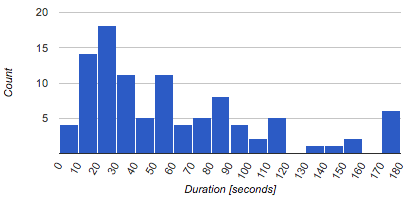
\includegraphics[width=18pc]{reaction-histogram-2016.png}
\caption{\label{reaction-histogram}Reaction time histogram.}
\end{minipage}\hspace{2pc}%
\begin{minipage}{18pc}
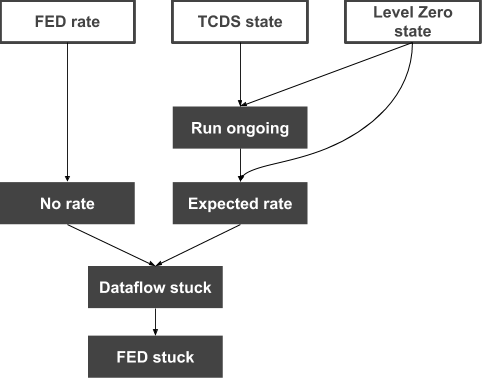
\includegraphics[width=18pc]{logic-module-hierarchy.png}
\caption{\label{subsetoflm}Subset of Logic Module hierarchy.}
\end{minipage} 
\end{figure}



\subsection{Minimizing external help}
In case the operators cannot fix the problem themselves they can always rely on help from DAQ on-call experts who are available 24/7. A scheme where operators cope with problems without the need for external help is desirable. Minimizing the number of these calls, especially outside working hours, without a deterioration of CMS efficiency is one of the goals of the project.


\subsection{Facilitating post mortem analysis}
After the problem occurs and is addressed, usually there is a lesson to be learnt to avoid similar problems in the future. Numerous monitoring systems enable access to data necessary to analyze the problem, albeit with some caveats. Some data are available after the problem has been resolved, some only while the problem is ongoing. The aim of the project is also to streamline the post mortem analysis by making both historic and real-time data easily available in the same way at any moment.

\section{Expert system and architecture}
Particular external forces influenced the design of the project and technologies used. Specifically no rule-based engine framework has been used to implement reasoning and define expert knowledge.

The system consists of three services. Firstly, the {\it Snapshot Service} aggregates all monitoring information into a snapshot and persists it. Secondly, the { \it Reasoning Service} applies the knowledge of the experts on the snapshots. Finally, the { \it Notification Manager } manages and delivers notifications, including e-mail and live suggestions and sound notifications in the control room. The { \it DAQExpert } brings all parts together in the form of a web application enabling browsing of the whole history of monitoring data to view the analysis and to manage notifications.

\subsection{External forces}
It is highly likely that the project's lifetime, like in many other cases at CERN, will be more than a~decade and the project will be maintained by different people over time. Thus, one of the main constraints was to avoid short-lived and highly specific technologies that would make it difficult for new team members to quickly become productive. It needs to be easy to understand and modifiable, requiring little effort to learn. Rule-based engines have beed evaluated in the past by the CMS DAQ group and were considered unsuitable due to the steep learning curve. Introducing additional languages was not an option. The solution needed to be based on the current skill set of the team members and as simple as possible.

Moreover, the nature of the project foresees frequent logic-related updates, possibly introduced by many authors. Whenever a new recovery solution is advised by sub-system experts the according knowledge needs to be introduced into the system. Finally, a high availability is essential, as each downtime of the system means no support for the operators and possibly extended downtime of CMS. 

As a result, the new expert framework has been designed from the ground up. It allows to define the knowledge in imperative language popular in the group - Java. The knowledge is organized in small independent Logic Modules that are building blocks of the system.


\subsection{Monitoring, aggregation and data flow}

There are multiple steps before information from data sources is available to the clients. The monitoring data sources are queried to get information about data taking health. There are multiple heterogenous sources of monitoring data. They differ not only in terms of what data is available, but also when and how quickly the data can be retrieved. Diagnosing the problems in data-flow in real time requires quick access to key information. Post mortem analysis requires access to all relevant data at any time. To enable both, a so-called snapshot of the system is taken periodically, approximately every 2 seconds. It contains all necessary information to identify and understand the problem. Thus, the first step was to aggregate all the information in snapshots that bring together both structural data and instantaneous states of all components. The scope of the snapshot has been designed to give the full picture of the system's state at a given moment. Both real-time and post-mortem analysis are based on the same data from the snapshots.

While the snapshot is persisted for possible post-mortem analysis it is simultaneously sent to the {\it Reasoning Service} for real time analysis. As a result of the analysis, notifications may be yielded that will be later dispatched by the {\it Notification Service} and delivered to the clients. On the way, all of the services persist their results enabling browsing of historic data.


\subsection{Knowledge definition}
Its common in the industry that the expert knowledge is defined in a declarative language. For instance, in a form of if-then-else rules expressed in a high-level rules language. As a result of external forces, this way of defining knowledge has not been used. The new custom made framework based on {\it Logic Modules} has been introduced. A {\it Logic Module} (hereinafter LM) is a~building block of {\it DAQExpert} expert logic. Each LM focuses on one thing: expressing a piece of knowledge about the DAQ system:


\begin{itemize}
\itemsep0em
\item each LM defines one condition,
\item the definition of condition is placed in the satisfy method,
\item the method returns true if condition is satisfied and false otherwise,
\item one LM can use results of another LM.
\end{itemize}

The knowledge defined in the LMs is used to find the optimal solution when a problem occurs in the data-flow. LMs operate on the snapshot and verify that key parameters are in expected states or in specified value ranges. As LMs may use outputs of other LMs, there is a predefined order of firing them. Figure~\ref{subsetoflm} presents a subset of LMs responsible for identifying one of many problems that may occur during data-taking. In the example there are five LMs and three parameters being monitored. The LMs are fired in top-down order allowing LMs to rely on others as indicated by arrows.


A LM may play two roles: it might be a sub-step of the analysis ({\it Expected rate}, {\it No rate}, {\it Dataflow stuck}) or final step of the analysis ({\it Front End Driver (FED) stuck}) delivering a description of the condition and a recovery suggestion. Finding optimal recovery from a given condition in this hierarchy means that the following chain of LMs was activated:

\begin{itemize}
\item {\it Run ongoing} -  there was a run started according to the {\it TCDS state} (TCDS - Timing and Control Distribution System) and{ \it Level Zero state} (Level Zero - Top level node in the run control system),
\item{\it No rate} - the average {\it FED rate} was 0, there was no data flowing
\item{\it Expected rate} - the {\it TCDS state}  and {\it Level Zero state} indicate that no recovery action is being issued at the moment, all subsystems are running and the rate is expected to be non-zero, it also checks if there is currently a run ongoing using the output of the {\it Run ongoing} LM
\item {\it Dataflow stuck} - this summarizes outputs of two LMs: {\it No rate} and {\it Expected rate}, it's activated when two related LMs are active, meaning that the data-flow is stuck,
\item {\it FED stuck} - starts the analysis when there is {\it Dataflow stuck}, it performs specific checks that reveal the specific FED stuck, causing the data-flow to be stuck, this LM identifies precisely the problem thus it contains final instructions for the operator, including a detailed description of the problem and a recovery suggestion.
\end{itemize}



\section{Results}

The current version of the service (2.9.0) improves all of the outlined areas. Operators of the DAQ system at CMS now have at their disposal a tool delivering recovery action suggestions in real-time - the Dashboard (see figure~\ref{dashboard-tool}). Whenever a problem occurs the tool shows the description of the problem and the optimal steps to recover. It helps shifters to take correct decisions, reducing both reaction time and need of external human expert help.

Measuring the success of the project was quite a challenging task. The ultimate goal is to increase the efficiency of data-taking at the CMS. However, the overall efficiency is not an adequate parameter as there are many different factors that interfere. The detector is constantly being improved, there were major upgrades in both hardware and software that influenced the final efficiency of CMS. The feedback of operators and human experts is important as they are the target user groups of the system. As much as they appreciate the new system, the subjective verbal feedback cannot be used as a measure of success as it is not quantitive. Three parameters have been identified to adequately represent the success of the project: accuracy of the recovery action selection, reaction time of the operators and demand of external help. They are practically independent of other factors, which makes them a reliable means of comparison.

The DAQExpert was introduced in mid 2016, but operators were instructed to use it in early 2017. All comparisons are based on {\it comparison period} (see section \ref{reaction-section}), which gives four months from 2016 where there was no {\it DAQExpert} support and two months from 2017 where the support was available. 


\subsection{Intervention time}

Improvement was mostly observed in the number of optimal recovery decisions taken by operators in case of data-flow upsets. As stated before, the recovery time is the majority of the total intervention time (82\%), thus it is essential to minimize it by choosing the most appropriate and time-efficient recovery actions (optimal recovery actions). 

There are two main categories of recovery actions: heavy - lasting usually for 3-4 minutes, initiated by e.g. stopping the run; and light - lasting 7-10 seconds implemented with commands through the TTC system. Suboptimal decisions mean unnecessary time spent on recovery or irrelevant actions that will not solve the problem leading to similar problematic condition after its completion. On average it means that each suboptimal decision adds between 93 and 125 seconds of overhead to the recovery time.

In 2016, during data-taking, operators had no guidance and out of 36 data-taking failures, 32 times the optimal decision was taken. In 2017 there were 29 data-taking failures and all of the decisions were optimal.

The reaction time is a secondary area to improve, as it is a minor part of the total intervention time - 18\%. There is a large variation depending on individual operator capabilities. The reaction time has slightly improved from 67 seconds in 2016 to 60 seconds in 2017. This is an area where the human factor plays an important role and bypassing the operators will certainly assure better results.


\subsection{Non-quantitative results}
An improvement in the post-mortem analysis has also been made. In the case of more demanding data-flow upsets, where further investigation is required, the{ \it DAQExpert} streamlines the chores of human experts. First, the go-back in time functions have been introduced that enable human experts to access the historic data easily with the {\it Browser} tool, shown in figure~\ref {browser-tool}. Secondly, there are more data available to support post-mortem analysis than ever before. All parameters of the system are kept for some period of time when debugging demand is more likely.



\begin{figure}[h]
\begin{minipage}{18pc}
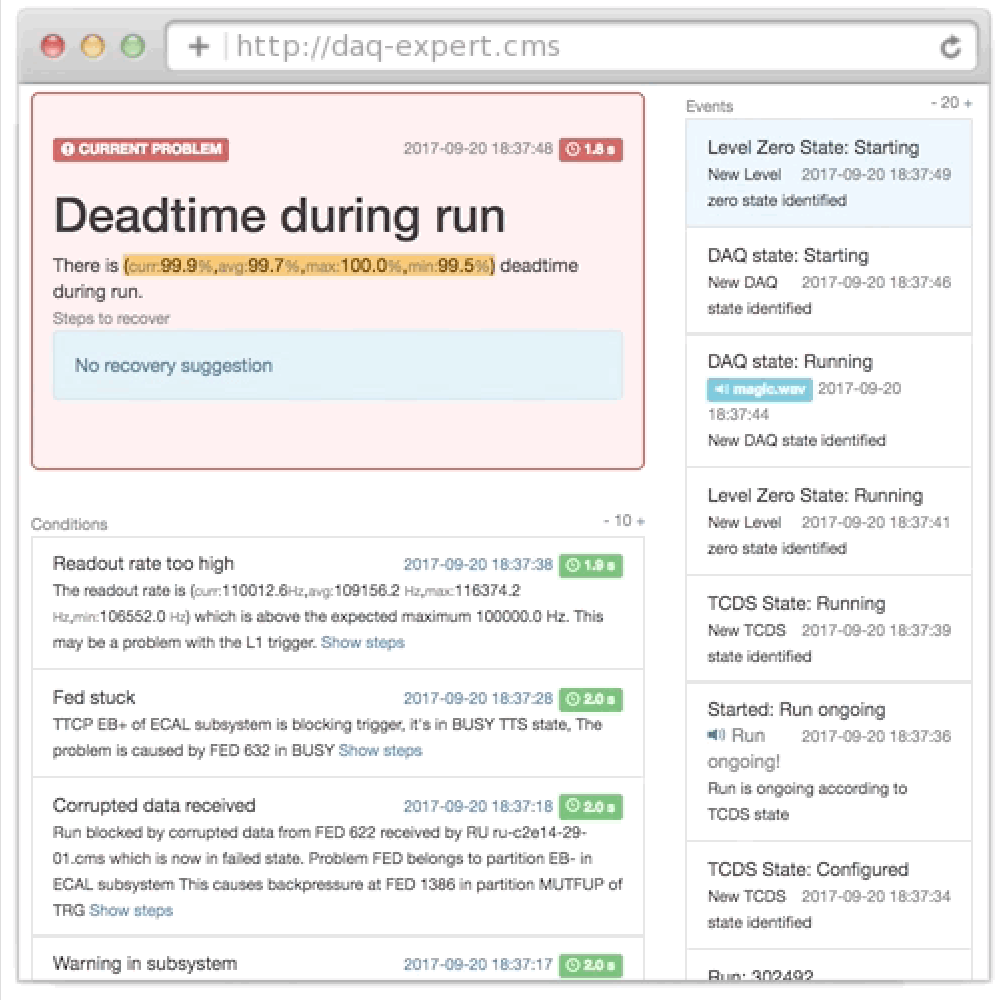
\includegraphics[width=18pc]{tool-dashboard2.png}
\caption{\label{dashboard-tool}Dashboard - tool to show suggestions in real time.}
\end{minipage} \hspace{2pc}%
\begin{minipage}{18pc}
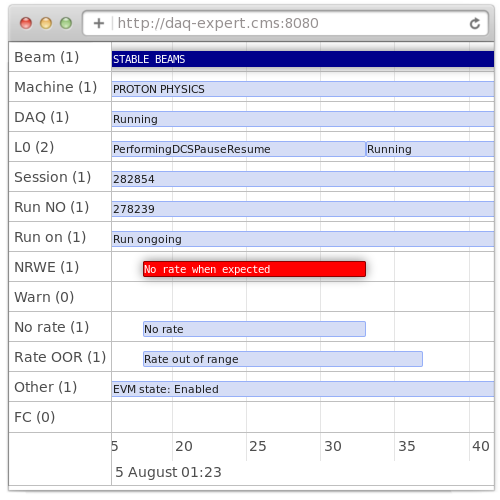
\includegraphics[width=18pc]{tool-browser2.png}
\caption{\label{browser-tool}Browser - tool to browse in time to enable post mortem analysis.}
\end{minipage}
\end{figure}


\subsection{Summary}
Both quantitative and qualitative results were presented in this chapter. The recovery action selection accuracy was improved by introducing the expert system. There were no suboptimal recovery decisions observed after deployment of {\it DAQExpert}. Whereas, before they occurred 11\% of the time. Additionally the reaction time shrunk from 67 to 60 seconds, which means that the total intervention time, including reaction time and recovery procedure time, is now shorter by at least 10 seconds. One major improvement to be implemented in the future is to bypass the operator whenever possible. This will shrink the reaction time to a few seconds.
External help demand has not yet been quantified. This area is of great interest for on-call human experts as it has the potential to limit the demand on their expertise. The number of phone calls (normalized by the number of problems) to the on-call experts before and after {\it DAQExpert} introduction may reveal trends in this area.


\section*{References}
\begin{thebibliography}{9}

\bibitem{cms} CMS Collaboration, JINST 3 S08004 (2008)
\end{thebibliography}





\end{document}


